% -*- TeX -*- -*- UK -*- -*- Soft -*-


\chapter{Dask}
\label{chap:Dask}

\section{Overview}
\label{sec:DaskOverview}


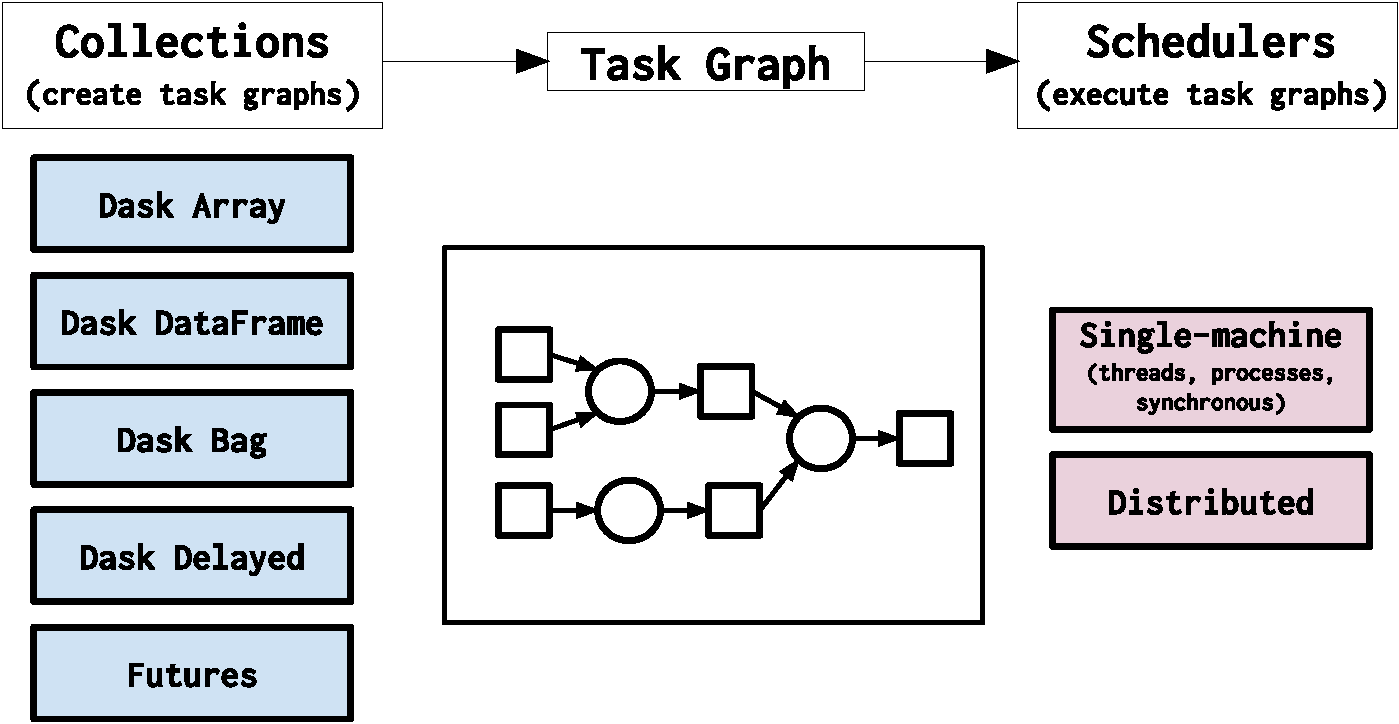
\includegraphics[width=.6\textwidth]{pic/dask-overview}

Dask \cite{daskhomepage2020} is a flexible library for parallel computing in Python.
Dask is composed of these parts:
\begin{enumerate}
\item Scheduler: Dynamic task scheduling optimized for computation. This is similar to Airflow, Luigi, Celery, or Make, but optimized for interactive computational workloads.
\item Graphs: Dask represents parallel computations with task graphs.  Working directly with dask graphs is rare, unless you intend to develop new modules with Dask. Dask graphs are created internally and most users don't ever see a graph.
\item Collections: ``Big Data'' collections like parallel arrays, dataframes, and lists that extend common interfaces like NumPy, Pandas, or Python iterators to larger-than-memory or distributed environments. These parallel collections run on top of dynamic task schedulers.
\end{enumerate}

The graph and collections functionalities are very powerful but not used in the \libradtrandask{} module. These topics are not further considered here.

Dask installs  conveniently  on a laptop, a desktop or a cluster computer. Dask can scale to a cluster of 100s of machines. This ease of transition between single-machine to moderate cluster enables users to both start simple and grow when necessary.  The \libradtrandask{} module uses the Dask scheduler to run \libradtran{} on a Linux computer, serving locally or to remote computers.

\section{Dask as Server}

The client Client-Server design pattern is generally used in the context where any number of clients, running on many different (weaker) computers can access the centralised server that is highly optimised to perform a specific set of functions very efficiently.  A common instance of this pattern is in enterprise database systems such as SAP or PeopleSoft. The clients have a small footprint (called 'thin', perhaps even just a browser), with most of the functionality in the main server (often with big databases and high processing capability).

A cloud service is any service made available to users on demand via the Internet from a cloud computing provider's servers as opposed to being provided from a company's own on-premises servers. Cloud services are designed to provide easy, scalable access to applications, resources and services, and are fully managed by a cloud services provider.
In the context of this document, consider the cloud service as a massively parallel computer providing computing and/or storage via the internet.

Dask is neither of the above, it is a technology that enables parallel computation, either on the local computer, on other computers on a private network or even in a cloud service.



but could in principle use a cloud serv

Dask is designed to support parallel computation, not as a general purpose server. So wWhy use Dask for this purpose? 
